\documentclass{standalone}
\usepackage{tikz}
\usetikzlibrary{through,calc, quotes,angles}

\begin{document}
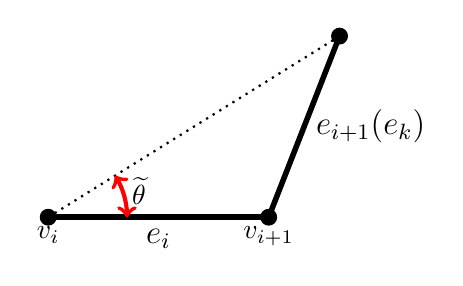
\begin{tikzpicture}
  \coordinate (A) at (-4, -0.8);
  \node at (A) [below] {$v_i$};
  \coordinate (B) at (-1.2, -0.8);
  \node at (B) [below] {$v_{i+1}$};
  \coordinate (C) at (-0.3, 1.5);
  \draw [fill] (A) circle [radius=0.1];
  \draw [fill] (B) circle [radius=0.1];
  \draw [fill] (C) circle [radius=0.1];
  \draw [thick, line width=2pt](A) -- (B) node [midway, below, font = \large] {$e_i$};
  \draw [thick, line width=2pt](B) -- (C) node [midway, right, font = \large] {$e_{i+1}(e_{k})$};
  \draw[thick, dotted] (A) -- (C);
  \draw pic["$\widetilde{\theta}$",draw=red,<->,angle eccentricity=1.2,angle radius=1cm, line width=1.5pt] {angle=B--A--C};
\end{tikzpicture}
\end{document}
